\documentclass[11pt]{jarticle}
\usepackage[dvipdfmx]{graphicx}
\usepackage{float}
\setlength{\textheight}{43\baselineskip}
\addtolength{\textheight}{\topskip}
\setlength{\textheight}{21\footskip}
\setlength{\textwidth}{42zw}
\setlength{\hoffset}{-5zw}
\usepackage{amsmath,amssymb,bm}
%
\usepackage{fancyhdr} %ヘッダー
\pagestyle{fancy}
\rhead{物理数学 \ 2016.05.09}
\renewcommand{\headrulewidth}{0pt} %ヘッダーラインを打ち出さない
%
\def \bun#1#2{\left(\frac{#1}{#2}\right)} %括弧付き分数マクロ
\def \vec#1{\mbox{\boldmath $#1$}} %ベクトルマクロ
\def \rot{\nabla \times} %ローテーション
\def \div{\nabla \cdot} %ダイバージェンス
\def \intt{\int\!\!\!\int} %2重積分
\def \intf#1#2#3#4{\int_{#1}^{#2}\!\!\!\int_{#3}^{#4}} %2重積分範囲付き
\def \inttt{\int\!\!\!\int\!\!\!\int} %3重積分
\def \intff#1#2#3#4#5#6{\int_{#1}^{#2}\!\!\!\int_{#3}^{#4}\!\!\!\int_{#5}^{#6}} %3重積分範囲付き
%
%%------------------------------%%
\begin{document}
\begin{center}
{\Large
演習問題その9小テスト}\\
\ \\
\underline{学籍番号:          }, 
\underline{氏名:            }
\end{center}
\begin{enumerate}
%%-----(問題開始)-----%%
\item[1.]
等質量$m$のおもり1,2がバネにつながれている.各バネのバネ定数は全て同じ$k$である.以下の問いに答えよ.\\
\begin{figure}[htpb]
\begin{center}
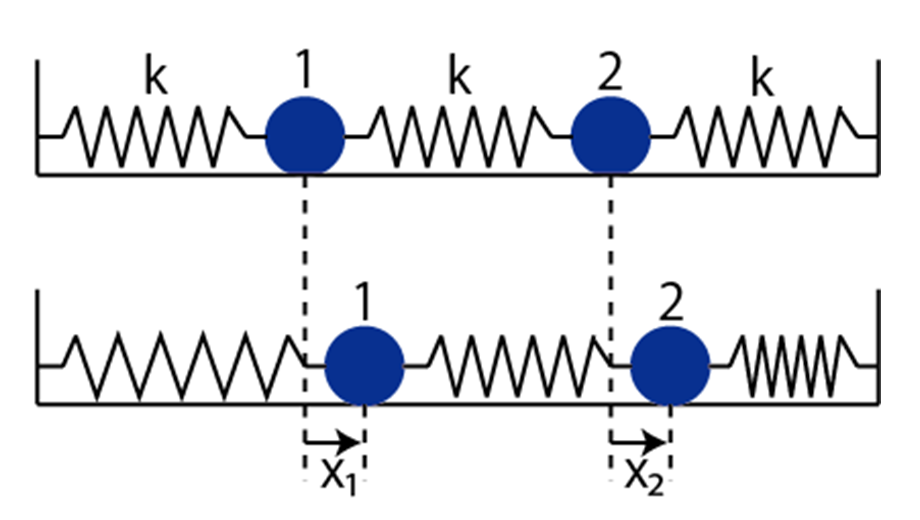
\includegraphics[scale=.20]{bane.png}
\end{center}
\end{figure}
\\
(1)$おもり1,2それぞれの平衡点からの変位をx_1,x_2としておもりの運動方程式を求めよ.$\\
(2)$x_1,x_2の一般解を求めよ.$


%%-----(問題終了)-----%%
\end{enumerate}


\newpage
%%------------------------------%%
%%-----(   解答ここから   )-----%%
\begin{center}
{\Large
演習問題その5小テスト 解答例}\\
\end{center}
\begin{enumerate}
\item[1.]
等質量$m$のおもり1,2がバネにつながれている.各バネのバネ定数は全て同じ$k$である.以下の問いに答えよ.\\
\begin{figure}[htpb]
\begin{center}
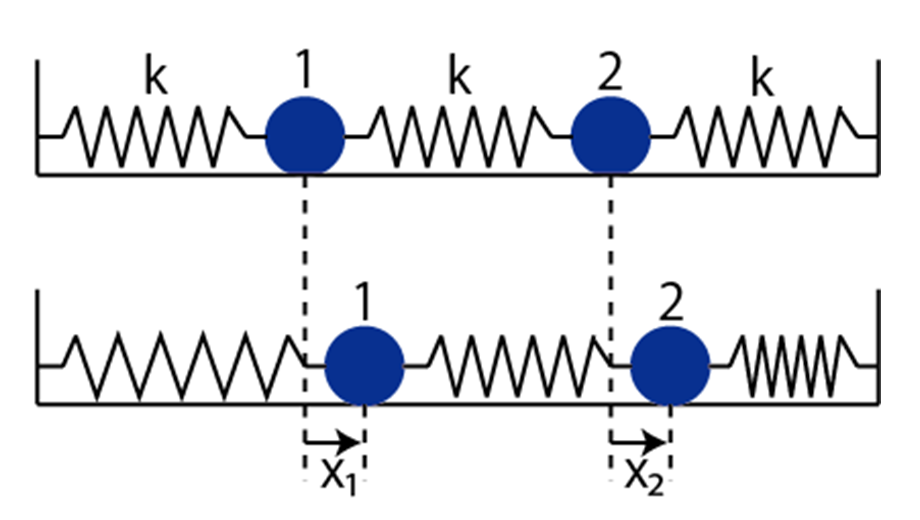
\includegraphics[scale=.20]{bane.png}
\end{center}
\end{figure}
\\
(1)$おもり1,2それぞれの平衡点からの変位をx_1,x_2としておもりの運動方程式を求めよ.$\\
(解答例)\\
\\
$\left\{ \begin{array}{l}
m\ddot{x_1}=-kx_1-k(x_1-x_2)=-2kx_1+kx_2 \\
m\ddot{x_2}=-kx_2+k(x_1-x_2)=kx_1-2kx_2
\end{array} \right.$\\
\\
(2)$x_1,x_2の一般解を求めよ.$\\
(解答例)\\
連立している式の和と差をとることにより、\\
\\
$\left\{ \begin{array}{l}
m(\ddot{x_1}+\ddot{x_2})=-k(x_1+x_2) \\
m(\ddot{x_1}-\ddot{x_2})=-3k(x_1-x_2)
\end{array} \right.$\\
よって、\\
$\left\{ \begin{array}{l}
x_1+x_2=a\cos({\omega}_1t+\alpha),\quad {\omega}_1=\sqrt{k/m} \\
x_1-x_2=b\cos({\omega}_2t+\beta),\quad {\omega}_2=\sqrt{3k/m}
\end{array} \right.$\\
$(ただし、a,b,\alpha ,\beta は定数)$\\
\\
したがって一般解は、
\begin{eqnarray*}
x_1=\frac{1}{2}a\cos({\omega}_1t+\alpha)+\frac{1}{2}b\cos({\omega}_2t+\beta)
\end{eqnarray*}
\begin{eqnarray*}
x_2=\frac{1}{2}a\cos({\omega}_1t+\alpha)-\frac{1}{2}b\cos({\omega}_2t+\beta)
\end{eqnarray*}

%%-----(解答終了)-----%%
\end{enumerate}

\newpage
(採点基準)10点満点、平均点7.1点\\
(1)が正解で+6点、(2)が正解で+4点。オマケで部分点をつけてある。

\end{document}
